\documentclass[12pt]{article}
\usepackage[utf8]{inputenc}
\usepackage[T1]{fontenc}
\usepackage[french]{babel}
\usepackage{graphicx}
\usepackage[top=3cm,bottom=2.5cm,left=2cm,right=2cm]{geometry}

\renewcommand{\contentsname}{Sommaire}
\renewcommand{\thesection}{\Roman{section}-}
\renewcommand{\thesubsection}{\Alph{subsection})}

\newcommand{\Octave}{GNU Octave }
\newcommand{\Matlab}{MATLAB\textsuperscript{\textregistered} }

\title{License SPI -- Projet Auralisation}
\author{Thomas \textsc{Lechat} \and Xin \textsc{Wang} \and Mathieu \textsc{Gaborit}}
\date{Note de synthèse 4 -- Décembre 2012}
\begin{document}

\maketitle

Pour la séance du 30 novembre, nous avons décidé de nous séparer pour avancer sur deux fronts en même temps : les moyens de comparaisons et le perfectionnement des scripts

\section{Mesures}% {{{1

Le but des mesures de cette séance était de fournir les données nécessaires à la comparaison de différents facteurs liés a l'auralisation: l'influence de la chaîne d'excitation et enfin l'utilisation de réponses impulsionnelles (RI) binaurales ou monaurale (la perception humaine étant binaurale).

Dans un premier temps, nous avons mesuré à nouveau la RI de la salle reverbérante pour avoir une réponse monaurale et binaurale prises dans les même conditions. Nous avons, de plus, pris 2 RI binaurales pour des positions de la tête différentes (face et un côté) afin de voir si la prise d'une RI suffit à localiser le son dans l'espace.

Une fois les RI acquises, nous avons enregistré le maximum de sons anéchoïques emis dans la salle afin de les comparer avec ceux que nous allons nous même convoluer. Nous avons donc enregistré des claquements de mains pour toutes les configurations de nos mesures ainsi que le debut d'une chanson pour une configuration binaurale et monorale.

\section{\Matlab / \Octave}% {{{1
\subsection{Normalisation} % {{{2

Au cours des séances précédentes, il a fallu souvent comparer des signaux (à partir de leur tracé).
Le fait de comparer des signaux n'ayant pas du tout la même dynamique était problématique.
Nous avons donc écrit une fonction \texttt{normalize(vect signal)} qui fait ça pour nous.

Même si la normalisation n'est pas forcément une opération compliquée (recherche du maximum \textit{via} \texttt{max()}
et division du vecteur par ce maximum), le fait de disposer d'une fonction pour le faire améliore grandement la
lisibilité du code (et donc sa maintenabilité).

\subsection{Comparaison entre \texttt{fftconv()} et \texttt{conv()}} % {{{2

Il a aussi été question d'utliser \texttt{fftconv()} en lieu et place de \texttt{conv()} pour faire nos convolutions.
Pour savoir si cette substitution avait un sens et ne nous faisait perdre de l'information (la transformée de Fourier
inverse n'étant pas parfaitement la réciproque de la transformée de Fourier, voir le principe de \texttt{fftconv()} en
figure~\ref{principe_fftconv}), nous avons mis en place une comparaison (voir figure~\ref{principe_comparaison}.) La
comparaison elle même est faite suivant la formule~\ref{formule_comp} (distance géométrique).

\begin{equation}
\label{formule_comp}
d = \sqrt{|s_1^2 - s_2^2|}
\end{equation}

Où :
\begin{itemize}
    \item $d$ est la distance
    \item $s_1$ et $s_2$ sont les deux signaux à comparer
\end{itemize}

\begin{figure}[h!]
\begin{center}
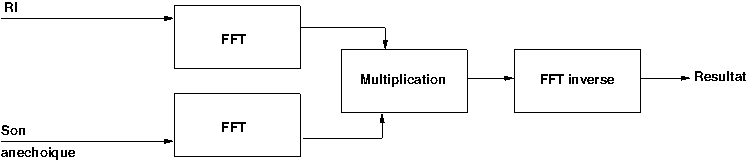
\includegraphics[width=15cm]{fftconv}
\caption{\label{principe_fftconv}Principe de la fonction fftconv()}
\end{center}
\end{figure}
\begin{figure}[h!]
\begin{center}
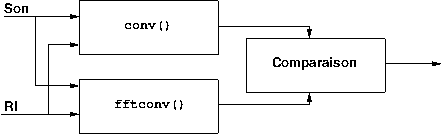
\includegraphics[width=15cm]{comparaison_principe}
\caption{\label{principe_comparaison}Principe de la comparaison mise en place. Une même RI et un même son sont convolués
en utilisant chacune des fonctions, puis comparées.}
\end{center}
\end{figure}

Le résultat de cette comparaison est tracé en figure~\ref{plot_comp}. On remarquera que l'axe des ordonnées pour la
troisième figure (distance entre les signaux) est graduée aux alentours de $10^{-7}$ ou $10^{-6}$. la différence entre
les deux procédés de convolution est donc très minime et négligeable au vu du gain de temps (énorme) que présente
l'utilisation de \texttt{fftconv()}.

\begin{figure}[h!]
\begin{center}
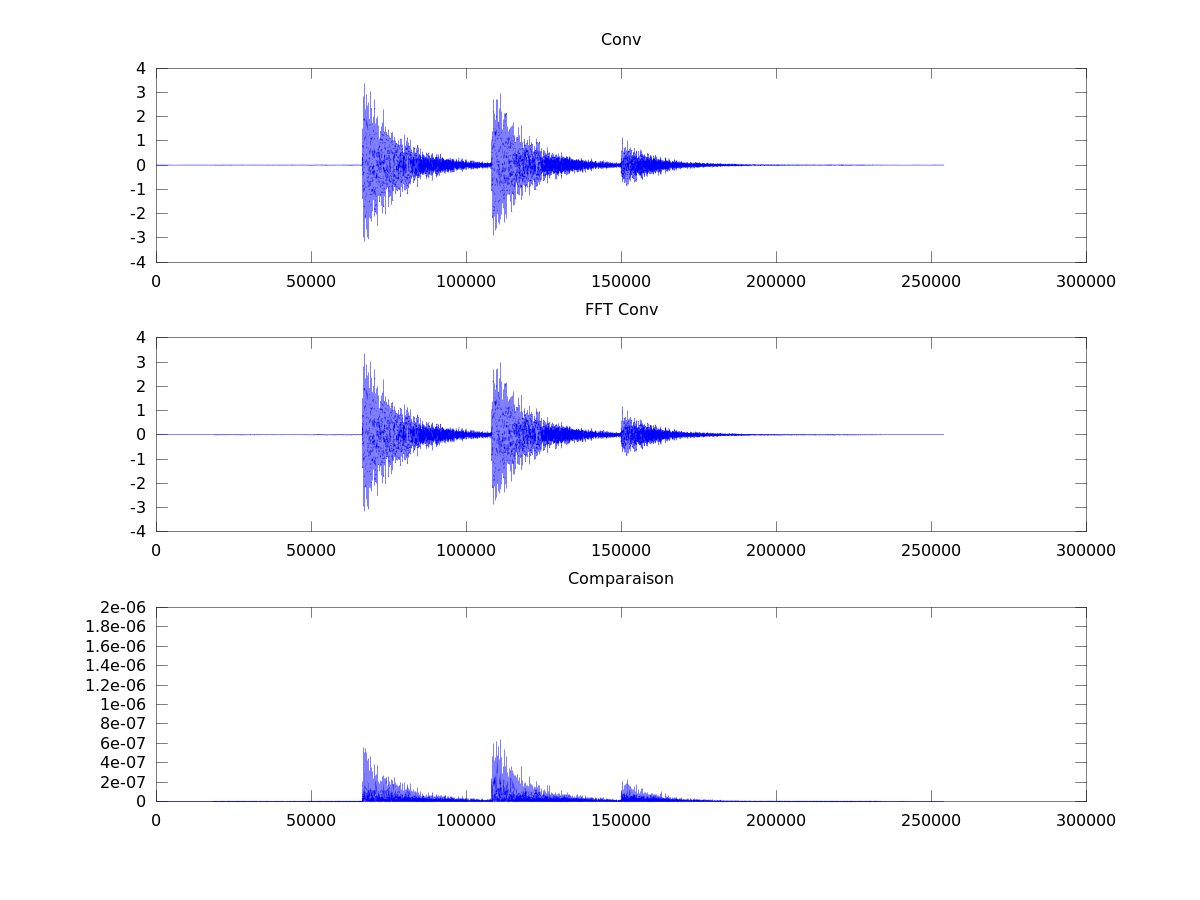
\includegraphics[width=10cm]{compare}
\caption{\label{plot_comp}Comparaison entre les résultats des deux fonctions. En haut : le signal résultant de
l'utilisation de \texttt{conv()} ; au centre : le signal obtenu avec \texttt{fftconv()} et en bas la distance entre les
deux signaux résultants.}
\end{center}
\end{figure}

\subsection{Calage temporel} % {{{2

Il faudrait réussir à caler les signaux en temps (débuts synchrones) pour pouvoir plus facilement les comparer. A la fin
de la séance du 7/12, l'algorithme semblait marcher.

\section{Auralisation proprement dite} % {{{1

Nous avons enfin convolué les signaux anéchoïques avec les RI et les avons comparés avec les mesures de ces mêmes signaux convolués "naturellement". Les résultats sont plus que satisfaisant d'un point de vu perceptif: nous arrivons à localiser le son dans l'espace en convoluant avec l'une ou l'autre des reponses binaurales et dans tout les cas nous avons clairement l'impression de nous trouver dans une salle avec un temps de reverbération élevé.

\section{La semaine prochaine}% {{{1

La semaine prochaine, il faudra revenir sur la partie informatique avec notament :

\begin{itemize}
    \item la mise au point des convolutions (saturations, etc...);
    \item le calage temporel de signaux (suite et fin);
    \item l'implémentation d'un algorithme de comparaison de signaux (à définir).
\end{itemize}

Nous allons aussi chercher à améliorer le processus d'auralisation en essayant de prendre en compte la chaine d'excitation et de mesure.

% }}}
\end{document}
